\documentclass[12pt]{amsart}
\usepackage{amsthm}
\usepackage{graphicx}
\newcommand*\oct{\vcenter{\hbox{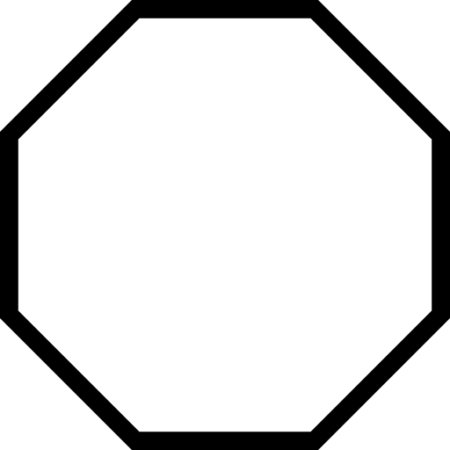
\includegraphics[width=.9em]{octagon.png}}}}
\newcommand{\F}{\mathcal{F}}
\newcommand{\Z}{\mathbb{Z}}

\newtheorem{theorem}{Theorem}
\newtheorem{lemma}{Lemma}
\newtheorem{corollary}{Corollary}

\theoremstyle{definition}
\newtheorem{definition}{Definition}

\title{Stopping Times}
\author{Robert Dougherty-Bliss and Charles Kenney}

\begin{document}
\maketitle

\begin{definition}
    A \emph{binary string of length $n$} is a tuple $(x_1, x_2, \dots, x_n)$
    where each $x_k$ is $0$ or $1$. Such a string is said to be \emph{stopped}
    at index $k$ if every index of the tuple in $(k / 2, k]$ is zero. The
    \emph{stopping time} of a binary string is the smallest $k$ such that the
    string is stopped at index $k$, or $\infty$ if no such $k$ exists. Note
    that, except $1$ and $\infty$, every stopping time is even.
\end{definition}

We are primarily interested in binary strings of length $n$ which have stopping
time $n$. Indeed, let $g(n)$ be the number of such strings. Our first goal is
to show that $g(n)$ satifies the recurrence
\begin{align*}
    g(1) &= g(2) = g(4) = 1 \\
    g(4n) &= 2 g(4n - 2) \\
    g(4n + 2) &= 2 g(4n) - g(2n).
\end{align*}
This will identify the sequence $a(n) = g(2n)$ as the
\emph{Narayana--Zidek--Capell numbers}, A2083 in the OEIS. This recurrence was
discovered thanks to the OEIS.

Our first definition discusses \emph{finite} binary strings, but it is more
convenient to work with \emph{infinite} binary strings which are nonzero in
only finitely many places. This is equivalent, and has the benefit that every
such infinite string has a finite stopping time when considered as a
sufficiently long, finite binary string.

\begin{definition}
    Let
    \begin{equation*}
        V = \bigoplus_{k=1}^\infty (\Z/2\Z)
    \end{equation*}
    be the direct sum of infinitely many copies of $\Z / 2\Z$. That is, the set
    of all infinite tuples $(x_1, x_2, x_3, \dots)$ where each $x_k$ is $0$ or
    $1$, and only finitely many are $1$. For each positive integer $k$, let
    $\oct_k$ be the set of elements of $V$ which are zero beyond position $k$
    and, when the first $k$ entries are regarded as a finite binary string,
    they have stopping time $k$. That is, $\oct_1 = \{0\} \subset V$,
    \begin{equation*}
        \oct_{2k} = \{v \in V : \forall j > k, v_j = 0, \text{ and } v \text{ has stopping time } 2k \}
    \end{equation*}
    and $\oct_{2k + 1} = \emptyset$ for every integer $k \geq 1$.
\end{definition}

It is clear that $g(n) = |\oct_n|$ for every positive integer $n$.

\begin{theorem}
    The sequence $g(n)$ satisfies the recurrence
    \begin{align*}
        g(1) &= g(2) = g(4) = 1 \\
        g(4n) &= 2 g(4n - 2) \\
        g(4n + 2) &= 2 g(4n) - g(2n).
    \end{align*}
\end{theorem}

% Todo
% Clean this up!
% Add details!
% (I [Robert] volunteer to do this.)
\begin{proof}
Define $e_0, e_1 : V \to V$ by
$$e_0(b) = \begin{cases} 0 \text{ if } b=0 \\ (b_1, ..., b_j, 0, 1, 0,0,...) \text{ if } b = (b_1, ..., b_j, 1, 0, 0, ...) \end{cases} $$
and
$$e_1(b) = \begin{cases} (1, 0,0,...) \text{ if } b=0 \\ (b_1, ..., b_j, 1, 1, 0,0,...) \text{ if } b=(b_1, ..., b_j, 1, 0, 0, ...). \end{cases} $$
Note that $e_0$ and $e_1$ are injective, $e_0(V) \cap e_1(V) = \emptyset,$ and $e_0(V) \cup e_1(V) = V.$
Let
$f:V \to V$
be given by
$$f(b) = \begin{cases} (b_1, ..., b_{j-1}, 1, 0,0,...) \text{ if } \exists j>0 \text{ s.t. } b = (b_1, ..., b_j, 1, 0,0,...) \\ 0 \text{ otherwise,} \end{cases}$$
so that $f \circ e_0 = f \circ e_1 = \text{id}_V.$
The map $e_1$ takes the element of $\oct_1$ to $\oct_2$, the element of $\oct_2$ to $\oct_4$, and in general for $k \geq 1,$
$$e_1 : \oct_{2k} \to \oct_{2k+2}.$$
Similarly, for $k \geq 2,$
$$e_0 : \oct_{4k-2} \to \oct_{4k}.$$
Let $\oct_{2k}^1 = \{(b_1, ..., b_{2k}, 1, 0,0,...) \in V \text{ s.t. } (b_1,...,b_{2k},0,0,...) \in \oct_{2k}\}.$
Then
$$e_0 : \oct_{4k} \to \oct_{4k+2} \cup \oct_{2k}^1$$
for all $k \geq 1.$
Now $e_0(\oct_{4k}) \supseteq \oct_{2k}^1,$ since if $b = (b_1, ..., b_{k-1}, 1, 0,0,...) \in \oct_{2k}$ then $(b_1, ..., b_{k-1}, 1, 0,0,...,0,1,0,0,...) \in \oct_{4k},$
where the final `1' is preceded by $k-1$ `0's.  
Finally, for all $k \geq 1,$
$$ e_0(\oct_{2k}) \cup e_1(\oct_{2k}) \supseteq \oct_{2k+2}.$$
\end{proof}

\end{document}
